\documentclass[14pt, fleqn, xcolor={dvipsnames, table}]{beamer}
\usepackage[T2A]{fontenc}
\usepackage[utf8]{inputenc}
\usepackage[english,russian]{babel}
\usepackage{amssymb,amsfonts,amsmath,mathtext}
\usepackage{cite,enumerate,float,indentfirst}
\usepackage{cancel}

\usepackage{tikz}                   
\usetikzlibrary{shadows}

% \usepackage{enumitem}
% \setitemize{label=\usebeamerfont*{itemize item}%
%   \usebeamercolor[fg]{itemize item}
%   \usebeamertemplate{itemize item}}

\graphicspath{{images/}}

\usetheme{Madrid}
\usecolortheme{seahorse}
\renewcommand{\CancelColor}{\color{red}}

\setbeamercolor{footline}{fg=Blue!50}
\setbeamertemplate{navigation symbols}{}
\setbeamertemplate{footline}{
  \leavevmode%
  \hbox{%
  \begin{beamercolorbox}[wd=.333333\paperwidth,ht=2.25ex,dp=1ex,center]{}%
    И. Кураленок, Н. Поваров, Яндекс
  \end{beamercolorbox}%
  \begin{beamercolorbox}[wd=.333333\paperwidth,ht=2.25ex,dp=1ex,center]{}%
    Санкт-Петербург, 2015
  \end{beamercolorbox}%
  \begin{beamercolorbox}[wd=.333333\paperwidth,ht=2.25ex,dp=1ex,right]{}%
  Стр. \insertframenumber{} из \inserttotalframenumber \hspace*{2ex}
  \end{beamercolorbox}}%
  \vskip0pt%
}
\newcommand\indentdisplays[1]{%
     \everydisplay{\addtolength\displayindent{#1}%
     \addtolength\displaywidth{-#1}}}
\newcommand{\itemi}{\item[\checkmark]}

\AtBeginSection[]
{  
 \addtocounter{framenumber}{-1}
 \begin{frame}<beamer>
   \frametitle{План}
   \small
   \tableofcontents[currentsection]
 \end{frame}
}

\title{Линейные модели: SVM\\\small{}}
\author[]{\small{%
И.~Куралёнок,
Н.~Поваров}}
\date{}

\begin{document}

\begin{frame}

\maketitle
\small
\begin{center}
\vspace{-60pt}
\normalsize {\color{red}Я}ндекс \\
\vspace{80pt}
\footnotesize СПб, 2015
\end{center}
\end{frame}


\section{Support vector machines}
\subsection{Идея метода}
\begin{frame}{SVM(воспоминания о былом)}
\begin{itemize}
  \item Последний из линейных методов, который мы рассмотрим подробно.
  \item Rocket science до конца 90-х, по крайней мере в задачах классификации.
\end{itemize}
\end{frame}

\begin{frame}{SVM на пальцах}
\begin{itemize}
  \item Максимальный зазор.
  \item Нелинейные преобразования.
\end{itemize}
\begin{center}
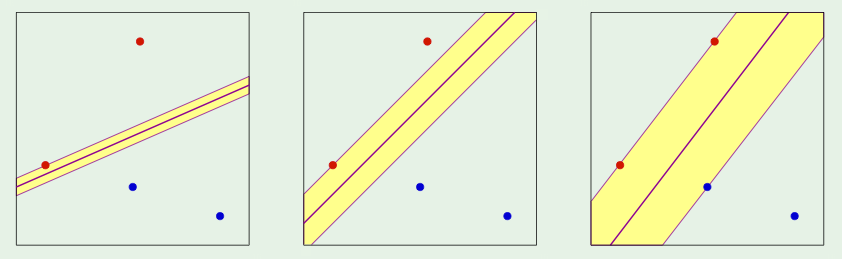
\includegraphics[width=0.9\textwidth]{SVM_1.png}
\end{center}
\end{frame}

\begin{frame}{Мысли вслух}
\begin{itemize}
  \item Почему большой зазор это хорошо?
  \item Какая $\beta$ максимизирует зазор? 
\end{itemize}
\end{frame}

\begin{frame}{Найдем ширину ``зазора'': геометрия}
\small
Есть две параллельные плоскости:
$$\left\{\begin{array}{l}
\beta^T x = a \\
\beta^T x = b
\end{array}\right.$$
проведем прямую, перпендикулярную этой плоскости: $y=\|\beta\| \frac{\beta}{\|\beta\|} t$. Пересечет она наши плоскости вот так:
$$\left\{\begin{array}{l}
\beta^T (\|\beta\| \frac{\beta}{\|\beta\|} t_a) = a \\
\beta^T (\|\beta\| \frac{\beta}{\|\beta\|} t_b) = b
\end{array}\right.$$
$$\left\{\begin{array}{l}
t_a = \frac{a}{\|\beta\|} \\
t_b = \frac{b}{\|\beta\|}
\end{array}\right.$$
тогда расстояние по полученной прямой: $|t_a - t_b| = \frac{|a-b|}{\|\beta\|}$ 
\end{frame}

\begin{frame}{Найдем ширину ``зазора'': мат. анализ}
\footnotesize
Решим оптимизацией:
$$
\min \frac{1}{2}\|x - y\|^2
$$
$$\left\{\begin{array}{l}
\beta^T x = a \\
\beta^T y = b
\end{array}\right.
$$
Перейдем к коэффициентам Лагранжа:
$$
\min \frac{1}{2}\|x - y\|^2 + \lambda_1 (\beta^Tx - a) + \lambda_2 (\beta^Ty - b)
$$
Найдем нули производных по всем переменным:
$$
\begin{array}{lll}
\left\{\begin{array}{l}
\beta^T x = a \\
\beta^T y = b \\ 
x - y + \lambda_1 \beta = 0 \\
x - y + \lambda_2 \beta = 0 \\
\end{array}\right.
&
\left\{\begin{array}{l}
\beta^T(x - y) = a - b \\
\lambda_1 = \lambda_2 \\
\|\beta\|\lambda_1 = b - a \\
\end{array}\right.
&
\left\{\begin{array}{l}
\lambda_1 = \lambda_2 = \frac{b-a}{\|\beta\|^2} \\
x - y = \frac{b - a}{\|\beta\|^2}\|\beta\|\left(\frac{\beta}{\|\beta\|}\right)
\end{array}\right.
\end{array}$$
\end{frame}

\begin{frame}{Возвращаясь к SVM}
\small
Теперь мы знаем что оптимизировать. Отнормируем разделяющие плоскости так:
$$
\left\{\begin{array}{l}
\beta^T x = b - 1 \\
\beta^T x = b + 1 \\
\end{array}\right.
$$
В этих терминах нас $|a - b|$ фиксированы и оптимизировать мы будем только $\beta$:
$$
\arg \min \frac{\|\beta\|}{2}
$$
Вот в таких условиях ($y_i \in \{-1,1\}$):
$$%\left\{
\begin{array}{l}
y_i(\beta^T x_i - b) \ge 1
\end{array}
%\right.$$
$$
\end{frame}

\subsection{Коэффициенты Лагранжа для решения задачи про максимальное расстояние}
\begin{frame}{По методу Лагранжа}
По теореме Куна-Таккера: \
$$
\mathcal{L} = \frac{1}{2}\|\beta\|^2 - \sum_{i=1}^m\lambda_i(y_i(\beta x_i - \beta_0) - 1), \lambda_i \ge 0
$$ 
$$
\left\{  
  \begin{array}{ll}  
  -\mathcal{L} = -\sum_{i=1}^m\lambda_i + \frac{1}{2}\sum_{i=1}^m\sum_{j=1}^m\lambda_i\lambda_j y_i y_j (x_i x_j) \\  
  \lambda_i \ge 0 & \\
  \sum_{i=1}^m\lambda_i y_i = 0
  \end{array}   
  \right.
$$
Тогда: \
$$\begin{array}{l}
\beta = \sum_{i=1}^m\lambda_i y_i x_i \\
\beta_0 = \beta x_i - y_i, \lambda_i > 0
\end{array}$$
\end{frame}

\begin{frame}{Чем стало легче?}
\begin{itemize}
  \item Адовые условия сменились простым $\lambda_i > 0$
  \item У нас получился квадрат количества точек
  \item Интересны только $(x_i, x_j)$ с которыми мы можем играться (kernel trick)!
\end{itemize}
\end{frame}
% Классные слайды http://www.cs.nyu.edu/~mohri/icml2011-tutorial/tutorial-icml2011-1.pdf
\begin{frame}{Напишем еще раз}
Вид двойственной задачи в случае линейной разделимости:
$$\begin{array}{l}
\arg \min_\lambda -\sum_{i=1}^m\lambda_i + \frac{1}{2}\sum_{i=1}^m\sum_{j=1}^m\lambda_i\lambda_j y_i y_j (x_i x_j) \\ 
\left\{  
  \begin{array}{ll}  
  \lambda_i \ge 0 & \\
  \sum_{i=1}^m\lambda_i y_i = 0
  \end{array}   
  \right.
\end{array}$$
Из решения двойственной задачи, можно получить решения прямой:
$$\begin{array}{l}
\beta = \sum_{i=1}^m\lambda_i y_i x_i \\
\beta_0 = \beta x_i - y_i, \lambda_i > 0
\end{array}$$
\end{frame}

\subsection{SVM в случае неразделимых множеств} % из вики

\begin{frame}{Мягкие границы}
\begin{center}
\includegraphics[height=0.4\textheight]{SoftMargins.png}
\end{center}
Перенесем точки-``нарушители'' на границу и добавим к целевой функции стоимость этого переноса:
$$\begin{array}{l}
\arg \min \|\beta\| + c\sum_i \xi_i \\
\left\{\begin{array}{l}
y_i(\beta^T x_i - \beta_0) + \xi_i \ge 1 \\
\xi_i \ge 0
\end{array}\right.
\end{array}$$
\end{frame}

\begin{frame}{Решение с мягкими границами}
\small
Прямая задача (заметим, что $dim(\lambda) = 2 m$):
$$\begin{array}{ll}
\arg \min_{\beta,\xi} \max_{\lambda} & \|\beta\| \\
  & + c\sum_i \xi_i \\
  & - \sum_i \lambda_{i} \left(y_i (\beta x_i - \beta_0) + \xi_i - 1\right) \\
  & - \sum_i \lambda_{i+m} \xi_i \\
\lambda_i > 0
\end{array}$$

Дуальная задача (Wolfe):
$$
\begin{array}{l}  
\arg \max_{\lambda} \sum_{i=1}^m\lambda_i - \frac{1}{2}\sum_{i=1}^m\sum_{j=1}^m\lambda_i\lambda_j y_i y_j (x_i x_j) \\  

\left\{\begin{array}{ll}  
  0 \le \lambda_i \le c & \\
  \sum_{i=1}^m\lambda_i y_i = 0
  \end{array}   
\right.
\end{array}
$$
Где-то мы такое (почти) уже видели. Решать такое надо условной оптимизацией, при этом задача не всегда выпукла (если $((x_i,x_j)) \succeq 0$).
\end{frame}

\begin{frame}{Нелинейные решения в SVM (Ядра)}
\small
Построим преобразование из исходного пространтсва в какое-то евклидово $\mathcal{H}$:
$$
\Phi: \mathbb{R}^n \to \mathcal{H}
$$
Тогда определим $(x_i, x_j) = (\Phi(x_i), \Phi(x_j))$. Что можно делать с ядрами \footnote{доказывается либо через определение, либо через теорему Мерцера}:
\begin{enumerate}
\footnotesize
  \item линейно комбинировать
  \item умножать
  \item комбинировать с функцией, раскладываемой в Тейлора с неотрицательными коэффициентами (например $e^x$)
  \item etc.
\end{enumerate}
В задаче можно поставить цель подобрать оптимальное ядро с помощью подобных преобразований.
\end{frame}

\begin{frame}{Известные Ядра}
\small
\begin{description}
  \item[Полиномиальные] $K(x,x^{'}) = (x^Tx^{'} + c)^d$ 
  \item[Гауссово (radial basis)] $K(x,x^{'}) = e^{-\gamma \|x - x^{'}\|_2^2}$ 
  \item[Сигмойдное (``Нейронное'')] $K(x,x^{'}) = tanh(k_1 (x,x^{'}) + k_2)$ 
\end{description}
В этом случае решение будет выглядеть иначе:
$$
h(x) = sign \left(\sum_i \lambda_i y_i (K(x_i, x) + \beta_0)\right)
$$
Заметим, что можно выкинуть все точки в которых $\lambda_i = 0$ (это какие?).
\end{frame}

\begin{frame}{Как подобрать ядро для решения задачи?}
\begin{enumerate}
\item Cross-fold
\item Исследование топологии $\Phi(x)$ \\
\small напримир, точки одного класса должны быть поближе, другого --- подальше.
\end{enumerate}
\end{frame}

\subsection{Сведение SVM к линейной системе с регуляризацией} % из книжки

\begin{frame}{SVM и регуляризация}
\small
Вспомним как выглядит наша решающая функция (без ядер): $h(x) = sign(x^T \beta + \beta_0)$. Тогда проблему можно переформулировать так:
$$
\min \sum_i (1 - y_i h(x_i))_+ + \frac{\lambda}{2} \|\beta\|^2
$$
А это минимизация hinge loss с $l_2$ регуляризацией. Теперь тоже самое, но с ядрами, $h(x) = sign \left(\sum_i \lambda_i y_i (K(x_i, x) + \beta_0)\right)$:
$$
\min \sum_i (1 - y_i h(x_i))_+ + \frac{\lambda}{2} \beta^T K \beta
$$
где $K : k_{ij} = K(x_i, x_j)$. Нас никто не ограничивает hinge loss, можно все тоже самое, но с любым другим лосем!
\end{frame}

\subsection{Регрессия в ядрах}
\begin{frame}{Kernel Ridge Regression}
\small
Если применима к любым функциям потерь, то почему не к $l_q$? Рассмотрим задачу оптимизации:
$$\begin{array}{l}
\min \sum \xi^2 \\
\left\{\begin{array}{l}
  y_i - \beta^T \phi(x_i) = \xi_i, \forall i \\
  \|\beta\| \le B
\end{array}\right.
\end{array}$$

Такое мы уже делали, поэтому приведу лишь результат ($\lambda = \lambda(B)$):
$$
\beta^* = 2 \lambda \left(K + \lambda E\right)^{-1}y
$$
\end{frame}

%\subsection{Простая оптимизация SVM} % ? из головы /machinelearning.ru
\section{Построение мультиклассификатора} % best 10 years paper award ICML2010
\begin{frame}{Как построить мультиклассификатор?}
\begin{itemize}
  \item Выберем очки для каждого класса и сведем задачу к регрессии
  \item Один против всех в количестве $k$ штук
  \item Построим одновременно несколько классификаторов с условием их соотношения (Multi-logit)
  \item Построим классификаторы для всех пар
  \item Есть еще идеи?
\end{itemize}
\end{frame}

\begin{frame}{Reducing multiclass to binary}
\small
E.L.~Alwien, R.E.~Schapire, Y.~Singer предложили интересную альтернативу:
Введем модельную матрицу $\mathcal{M} \in \{-1,0,1\}^{k\times l}$. Для каждого столбца подберем функцию бинарной классификации, отделяющую $+1$ от $-1$.
Решим исходную задачу одним из двух способов:
$$
d_H(c, f(x), \mathcal{M}) = \sum_{s = 1}^l\left({1 - sign(m_{cs} f_s(x)) \over 2}\right)
$$
$$
d_L(c, f(x), \mathcal{M}) = \sum_{s = 1}^l L(m_{cs} f_s(x))
$$
Теперь вопрос свелся к тому как найти оптимальный $\mathcal{M}$.
\end{frame}

\begin{frame}{Что мы узнали в прошлый раз I}
\small
\begin{itemize}
  \item Было бы классно найти такую плоскость, которая сильнее всего поделит на классы
  \item Если множества линейно разделимы, то надо минимизировать $\|\beta\|$
  \item Если перейти к дуальной задаче, зависимость от $x$ окажется только через скалярные произведения, которые мы можем ``организовать'' по своему разумению
  \item В дуальном решении условия очень просты и можно организовать безусловную оптимизацию заменой переменных
  \item Количество компонент оптимизации пропорционально квадрату количества точек, что много
\end{itemize}
\end{frame}

\begin{frame}{Что мы сегодня узнали II}
\small
\begin{itemize}
  \item SVM можно делать в случае линейной неразделимости
  \item Формулы получаются почти такие же, но еще и с верхней границей на $\lambda$
  \item В SVM есть ядра, их можно подбирать, однако решение в этом случае включает все граничные точки из-за того, что $\Psi$ не определено в явном виде
  \item SVM можно рассматривать как минимизацию hindge loss с регуляризацией по Тихонову
\end{itemize}
\end{frame}

\begin{frame}{Что мы сегодня узнали III}
\begin{itemize}
  \item На ядрах можно делать не только SVM, но и регрессию
  \item Несколько способов построения мультиклассификатора и их обобщение
\end{itemize}
\end{frame}


\end{document}
